% Wie eingangs erwähnt, definieren die Anforderungen, was das System zu leisten
% hat, während die Funktionalitä-ten definieren, wie das System diese
% gewährleistet.
\chapter{Interface-Design}
\label{chapter-design}
Neben den inhaltlichen Funktionalitäten ist im menschzentrierten
Gestaltungsprozess vor allem das Interface-Design und die Gestaltung der
Komponenten von zentraler Bedeutung \cite{DINISO9241} (DIN EN ISO 9241-210,
2011). Bei der Konzeption des Designs sollten die erarbeiteten Funktionalitäten
aus \ref{chapter-konzept} berücksichtigt werden. Folglich sollten die in
\ref{section:Nutzenden} erarbeiteten Nutzenden die Gestaltungslösungen verstehen
und bedienen können.

Die Medieninformatik bietet viele Methoden und Vorgehensweisen zur menschzentrierten Gestaltung
\cite{HerczegIDE2009}. Im Rahmen der Arbeit wurde vor allem Prototyping in verschiedenen Formen
eingesetzt \cite{HerczegMDI2009}. Des Weiteren wurden die Zehn Usability Heuristiken nach
\citeA{nielsen_enhancing_1994} bei der Entwicklung stets beachtet, um Kriterien der
Gebrauchstauglichkeit zu addressieren. Eine ausführliche Aufzählung der Heuristiken befindet sich in
\ref{appendix:Heuristiken}. In der Gestaltung wurde nach der \enquote{Mobile First}-Strategie
gearbeitet (\anfref{R40}). Hierbei wird die Oberfläche zunächst für kleine Bildschirmflächen
entwickelt, um die Informationsdichte an diesen zu orientieren. Erst beim Erweitern der Fläche
werden zusätzliche Informationen entsprechend des verfügbaren Platzes angezeigt
\cite{kim_chapter_2013}. Bei der Anordnung der Komponenten wurde sich an den
\nameref{subsection:interview} genannten Anwendungen, wie zum Beispiel
Airbnb\footnote{\url{https://www.airbnb.de/}} und Otto\footnote{\url{https://www.otto.de/}}
orientiert. Des Weiteren wurden Tailwind UI\footnote{\url{https://tailwindui.com/components}} und
Headless UI\footnote{\url{https://headlessui.com/}} als Inspirationsquelle herangezogen, um die
Realisierung des Systems zu erleichtern.

Die erste Iteration des Interface-Designs umfasst Skizzen. Die Skizzen wurden
erstellt, um einen groben Überblick der verschiedenen Ansichten zu erhalten und
in \textit{Mockup}\footnote{\url{https://getmockup.app/}} umgesetzt. Während des
Designprozesses wurden die Skizzen mit
Figma\footnote{\url{https://www.figma.com/de/}} zu einem High-Fidelity-Prototyp
weiterentwickelt.

Im Rahmen dieses Kapitels werden die zentralen Ansichten und
Design-Entscheidungen erläutert. Eine Übersicht aller Entwürfe befindet sich im
(\label{appendix:digitaleMedien}).

\section{Iteratives Vorgehen}
Für die Tests wurden Usability-Spezifikationen aus Szenarien abgeleitet. Die
Szenarien beschreiben Aufgaben, welche als Vorlage in der Evaluation dienen
können \todo{Anhang, Quelle Scenario Based Design einfügen - auch, wenn
    nicht nach dem Prozess vorgegangen, ist es doch sicherlich eine gute Quelle, die
    man für die Entwicklung von Szenarien zitieren kann}. Um repetitive
Evaluationsergebnisse zu verhindern, wurden die Evaluationsergebnisse
kontinuierlich in die weitere Entwicklung eingearbeitet. \ref{table:e} stellt
die Evaluationsteilnehmenden mit IDs dar, welche in den folgenden Abschnitten
als Verweise verwendet werden.

\begin{table}[h]
    \centering
    \caption{Teilnehmende der Zwischenevaluation}
    \begin{tabular}{lll}
        \arrayrulecolor{maincolor}\hline
        \sffamily\color{maincolor}ID & \sffamily\color{maincolor}Alter &
        \sffamily\color{maincolor}Rolle
        \\
        \arrayrulecolor{maincolor}\hline
        E1                           & 19 - 25 J.                      &
        Medieninformatiker:in
        \\
        E2                           & 19 - 25 J.                      &
        Robotiker:in                                                     \\
        E3                           & 19 - 25 J.                      &
        Medieninformatiker:in, Hilfswissenschaftler:in                   \\
        E4                           & 19 - 25 J.                      &
        Medieninformatiker:in                                            \\
        E5                           & 19 - 25 J.                      &
        Medieninformatiker:in, Hilfswissenschaftler:in
        \\
        E6                           & 25 - 30 J.                      &
        Wissenschaftliche:r Mitarbeiter:in                               \\
        \arrayrulecolor{maincolor}\hline
    \end{tabular}
    \label{table:e}
\end{table}

\section{Designsprache}

Im Folgenden wird auf die Entwicklung der wichtigsten Komponenten und Ansichten
in der Interfacegestaltung eingegangen.

\subsection{Wortlaut}
Ein zentrales Problem des Prototyps war der konsistente Wortlaut (H2, H4, H5).
Insbesondere der Begriff \textit{Assets} konnte mehrfach nicht oder schlecht
interpretiert werden (E1, E2). Daraufhin wurden Vorschläge geliefert, wie
\textit{Material, Hardware, Systeme, Geräte}. Im weiteren Verlauf hat sich
\textit{Material} als präferierter Begriff herausgestellt (E3-E5). Des Weiteren
hat das \textit{Suchen nach Kriterien} für Missverständnisse in Verbindung mit
der ebenfalls existierenden \textit{Suche} ergeben (E1, E2). Daher wurden auch
hier verschiedene Begriffe wie
\textit{Auswahlhilfe, Suchhilfe, Kriterien-Suche, Kriterien-Hilfe, Auswahl nach Kriterien, Ausleih-Hilfe}
erarbeitet. Da die Funktion im Rahmen dieser Arbeit nicht realisiert wurde, ist die Entscheidung bei
diesen Begriffen ausstehend.\todo{Ausblick}

\subsection{Schrift}
Allgemein wurde die Schriftart nach Kriterien für eine gute Lesbarkeit, wie:
Erkennbarkeit, Unterscheidbarkeit und Offenheit betrachtet
\cite{kommunikationsdesign_leserlichinfo}. Außerdem wurde sich für die spätere
Realisierung der Typografie direkt an Tailwind
UI\footnote{\url{https://tailwindui.com/components}} orientiert und somit Segoe
UI gewählt (\ref{fig:schrift}).

\begin{figure}[h]
    \centering
    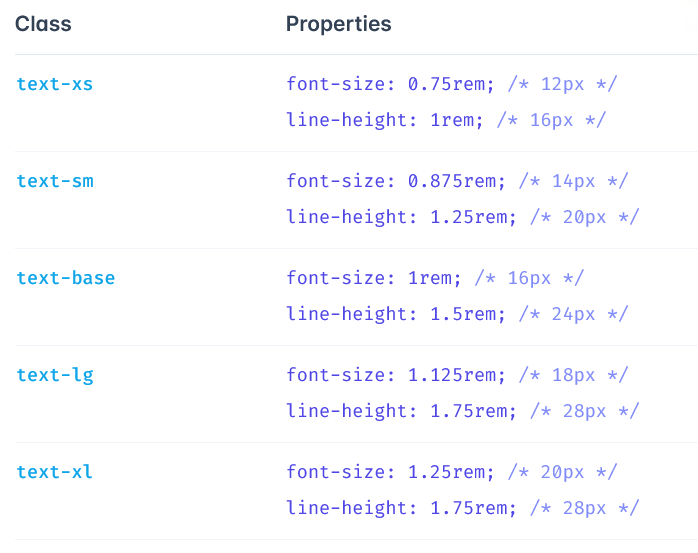
\includegraphics[scale=0.25]{Bilder/Prototyp/Screenshot 2022-09-27 at 15-07-24 Font Size - Tailwind CSS.png}
    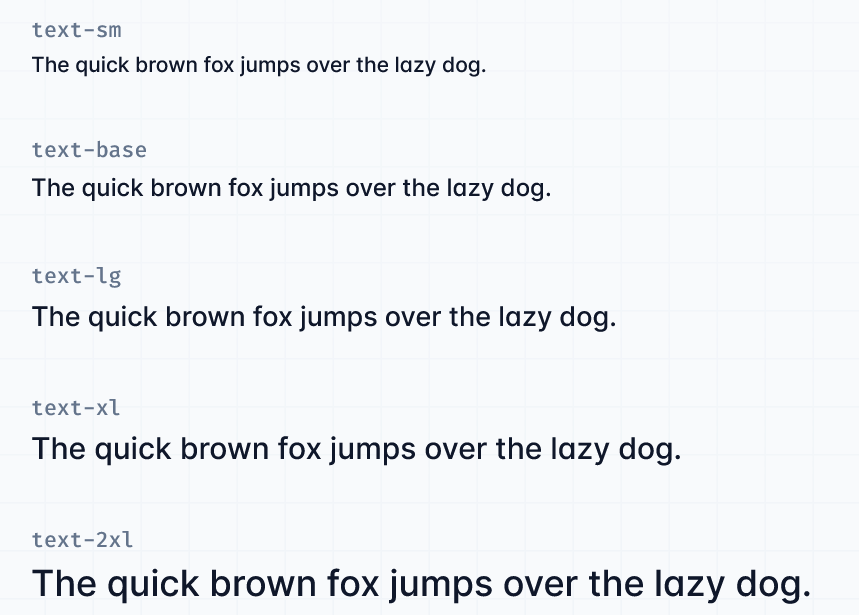
\includegraphics[scale=0.25]{Bilder/Prototyp/Screenshot 2022-09-27 at 15-07-37 Font Size - Tailwind CSS.png}
    \caption{Typografie von Tailwind UI}
    \label{fig:schrift}
\end{figure}


\subsection{Farbschema}
Die Farben der Anwendung (\ref{fig:farben}) werden nach dem 60-30-10 Prinzip genutzt
\cite{experience_using}. Hierbei stellt grau die Hauptfarbe dar, weiß die Sekundärfarbe und orange
die Akzentfarbe. Da die Anwendung für den Gebrauch am \ac{imis} entwickelt wird und die Farben des
Instituts sich auf Orange und das Universitäts-Blau beschränken, wurde sich nach einigen Vergleichen
für das Orange entschieden (E4, E5). Der dunkle Ton stellt die Textfarbe der Anwendung dar. Außerdem
wurde mit verschiedenen Graustuffen gearbeitet, um Interaktionen von Elementen zu verdeutlichen.

\begin{figure}[h]
    \centering
    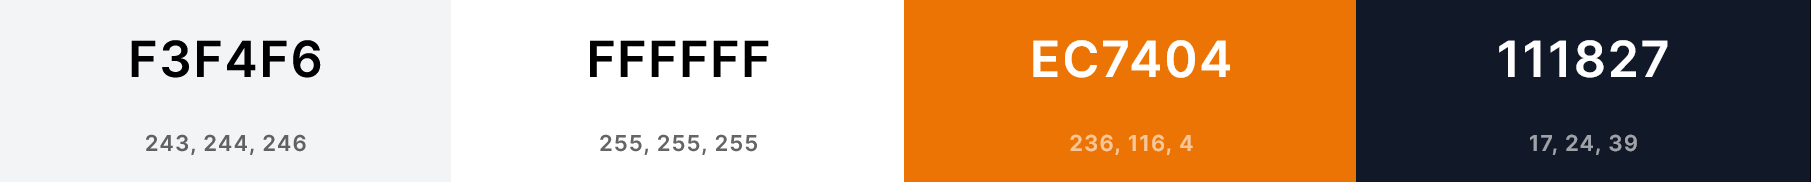
\includegraphics[scale=0.23]{Bilder/farben.png}
    \caption{Farbsystem des Interface-Designs}
    \label{fig:farben}
\end{figure}

\subsection{Dashboard}
Positiv wurde stets angemerkt, dass die Anwendung im allgemeinen verständlich
und \enquote{nicht überfordernd} wirkt (H8) (E1-6). Aufgrund des zu Beginn geringen
Inhalts auf der Startseite ist eine ansprechende und fokussierte Anordnungen der
Komponenten wichtig (H8). \ref{fig:home} zeigt die Entwicklung des Dashboards.
Ein wichtiger Punkt bildet die im linken Bild fehlende Orientierung (E1-4).
Außerdem wirkte die Ansicht durch die vielen einzelnen Elemente schnell
überladen (H8) (E1-2). Als Konsequenz wurde sich für eine Tab-Leiste entschieden.
Folglich ist die Seite auch bei mehr als drei Reservierungen übersichtlich (E4).
Sobald ein Asset ausgeliehen wurde, sollten die entsprechenden Informationen
(Status, Zeitraum, Ort) übersichtlich und schnell eingesehen werden können (H1)
(F-A-1). Dies ermöglicht die Kartenansicht, wobei eine Möglichkeit zum Löschen
und das Bearbeiten des Zeitraums erwünscht war und in der Realisierung
integriert wurde (E6).

Die Verwaltungsansicht, in welcher die Möglichkeit zum Aktualisieren des Status besteht, entspricht
zum Großteil dem Dashboard der Ausleihenden (H6) (F-V-1, F-V-2).

\begin{figure}[h]
    \centering
    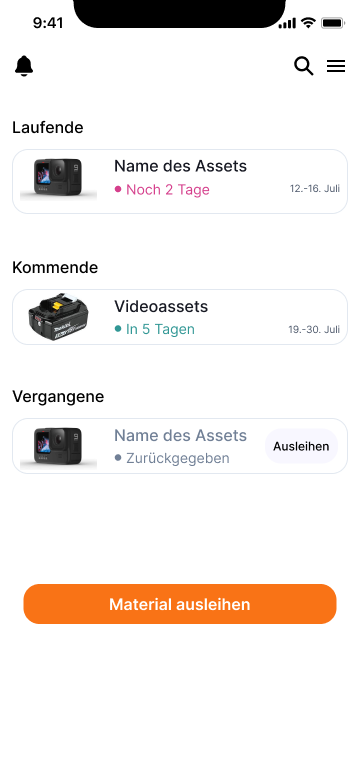
\includegraphics[scale=0.3]{Bilder/Prototyp/Start.png}\hspace{2em}
    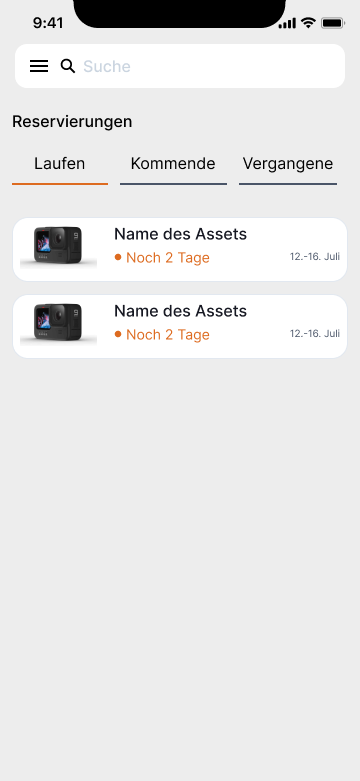
\includegraphics[scale=0.3]{Bilder/Prototyp/Neu/V2.png}
    \caption{Entwicklung des Dashboards in der mobilen Ansicht}
    \label{fig:home}
\end{figure}

\subsection{Navigation und Suchleiste}
In der Interface-Gestaltung gibt es verschiedene Möglichkeiten, die Navigation
bereitzustellen. Für den mobilen Kontext wurde eine Navigationsleiste am unteren
Bildschirmrand und ein Burgermenü in Erwägung gezogen. Für die
Desktop-Navigation wurde zwischen einer festen Navigationsleiste links und einer
Leiste oben abgewägt (\ref{fig:nav}). Am Ende wurde sich für eine
Navigationsleiste auf der linken Seite entschieden. Orientiert wurde sich
hierbei an bekannten Anwendungen mit ähnlichen Funktionalitäten (z. B. Google
Drive) und dem Material Design \cite{google_material_2022}. Die Umgangsweise mit
diesen Gestaltungslösungen ist bereits bekannt und somit übertragbar (H4, H6).
Daran anknüpfend wurde sich für eine integrierte Suchleiste entschieden, sodass
Nutzende jederzeit die Möglichkeit haben, nach Assets zu suchen
\cite{google_material_2022} (E4).


\begin{figure}[h]
    \centering
    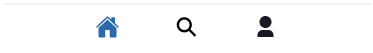
\includegraphics[scale=0.3]{Bilder/Prototyp/Property 1=Variant2.png}
    \hspace{2em} 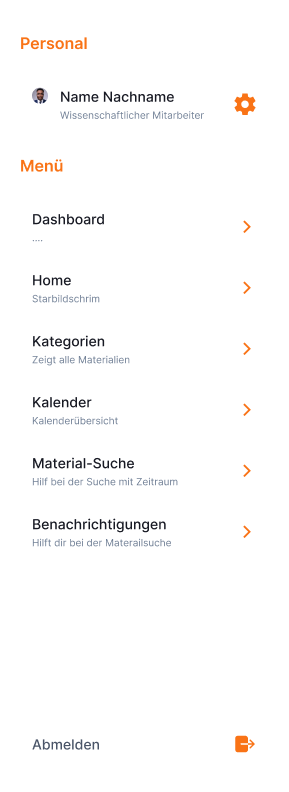
\includegraphics[scale=0.3]{Bilder/Prototyp/Menu.png}
    \hspace{2em}
    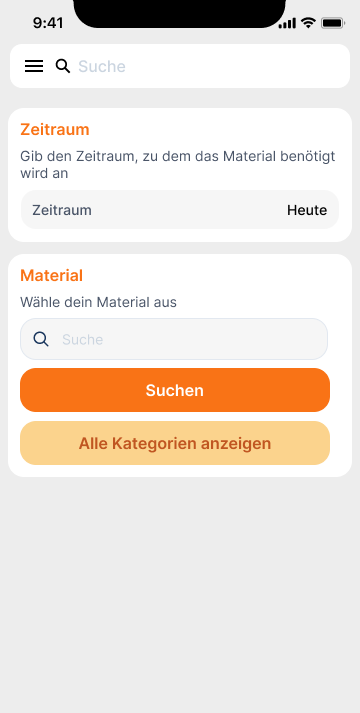
\includegraphics[scale=0.3]{Bilder/Prototyp/Neu/Suche V2.png}
    \caption{Navigationsmöglichkeiten und Suchleiste der mobilen Ansicht}
    \label{fig:nav}
\end{figure}

\subsection{Kategorien und Suche}
Bei der Übersicht der Kategorien wurde sich  ebenfalls an bekannte Anwendungen
mit ähnlichen Funktionen (z. B. Airbnb, Otto) orientiert (H4, H8). Dies führt
unter anderem dazu, dass Fehler besser vermieden werden können (H9).

Die Suche wurde der Anwendung Airbnb\footnote{\url{https://www.airbnb.de/}}
nachempfunden, da viele Nutzende den Reserviervorgang mit dieser Anwendung
assoziieren (H2, H4). Die Suche sollte durch das direkte Einstellen eines
Ausleihzeitraums Fehlern vorbeugen und die Verfügbarkeit anzeigen (H5) (F-VA-6).
\ref{fig:p1} zeigt die erste Version des High-Fidelity-Prototypen, bei welcher
ein Suchbutton fehlte. Zudem wurden die Vorschläge der angezeigten Kategorien
weniger genutzt und direkt auf die Suche oder \enquote{alle Kategorien Anzeigen}
geklickt. Daher wurden diese Elemente entsprechend angepasst (E1, E2, E4).

\begin{figure}[h]
    \centering
    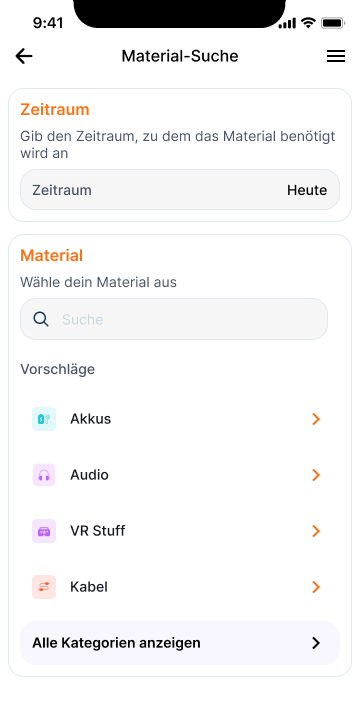
\includegraphics[scale=0.3]{Bilder/Prototyp/Suche.png}\hspace{2em}
    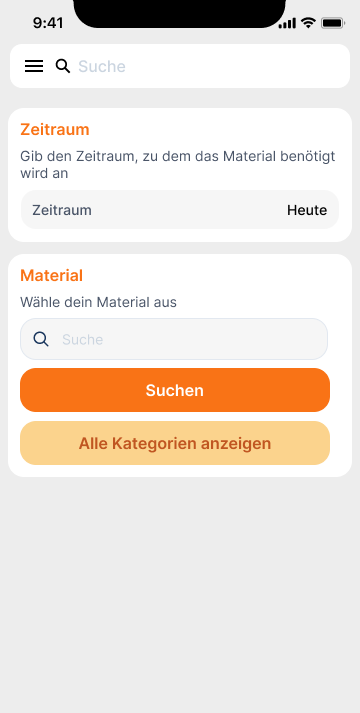
\includegraphics[scale=0.3]{Bilder/Prototyp/Neu/Suche V2.png}
    \caption{Entwicklung der Materialsuche in der mobilen Ansicht}
    \label{fig:p1}
\end{figure}

Für die Unteransicht wurde sich für eine Kartenansicht entschieden
(\ref{fig:ubersicht}). Diese ergab sich aus den bereits bekannten Vorgängen und
Interfaces von Online-Shops. Nutzenden wird mithilfe eines Bildes direkt
gezeigt, um was für ein Asset es sich handelt. Außerdem wird auch hier die
Assetverfügbarkeit mit eingebunden (H4, H8) (F-VA-3).

\begin{figure}[h]
    \centering
    \includegraphics[scale=0.3]{Bilder/Prototyp/Übersicht.png}\hspace{2em}
    \includegraphics[scale=0.3]{Bilder/Prototyp/Übersicht1.png}
    \caption{Entwicklung der Materialansicht (Kacheln) in der mobilen Ansicht}
    \label{fig:ubersicht}
\end{figure}

\subsection{Kalender}
Die Kalenderkomponente wurde lediglich als Skizze veranschaulicht
(\ref{fig:kalender}). Im High-Fidelity-Prototyp wurde sich bereits an der
Komponente
\textit{V-Calendar}\footnote{\url{https://vcalendar.io/layouts.html}}
orientiert, welche die wichtigsten Funktionen bereits implementiert und so die Realisierung
erleichtert.

Für den Kalender ist unter anderem die Möglichkeit zur Ausblendung von
Wochenendtagen wichtig, da zu diesen Zeitpunkten keine Ausleihe möglich ist (H1)
(F-VA-3). Außerdem sollten vergangene Tage nicht auswählbar sein. Weitere Punkte
wurden auch hier wiederholt mit der Anwendung Airbnb verglichen (H4, H7, H8) (E2-4).

Für Verleihende ist eine generelle Übersicht über einzelne Tage wichtig, um
Abholungen und Rückgaben von Assets besser planen zu können (F-V-4).

\subsection{Asset-Detailansicht und Reservierungen}
Die Ansicht der einzelnen Assets sollte insbesondere die Assetverfügbarkeit,
Funktionalitäten des Assets und die zuständige Person enthalten (F-VA-3, F-VA-4, F-VA-8).
\ref{fig:p3} zeigt die genannten Informationen. Es ergab sich, dass eine
Assetbeschreibung des Artikels zunächst nicht von Bedeutung sei (E6). Den
Ausleihzeitraum separat zur Abholung und Rückgabe anzeigen zu lassen, führte im
Verlauf häufig zu Verwirrung. Daher wurden die zeitlichen Daten auf die Abholung
und Rückgabe beschränkt (H5) (E5, E6).

\begin{figure}[h]
    \centering
    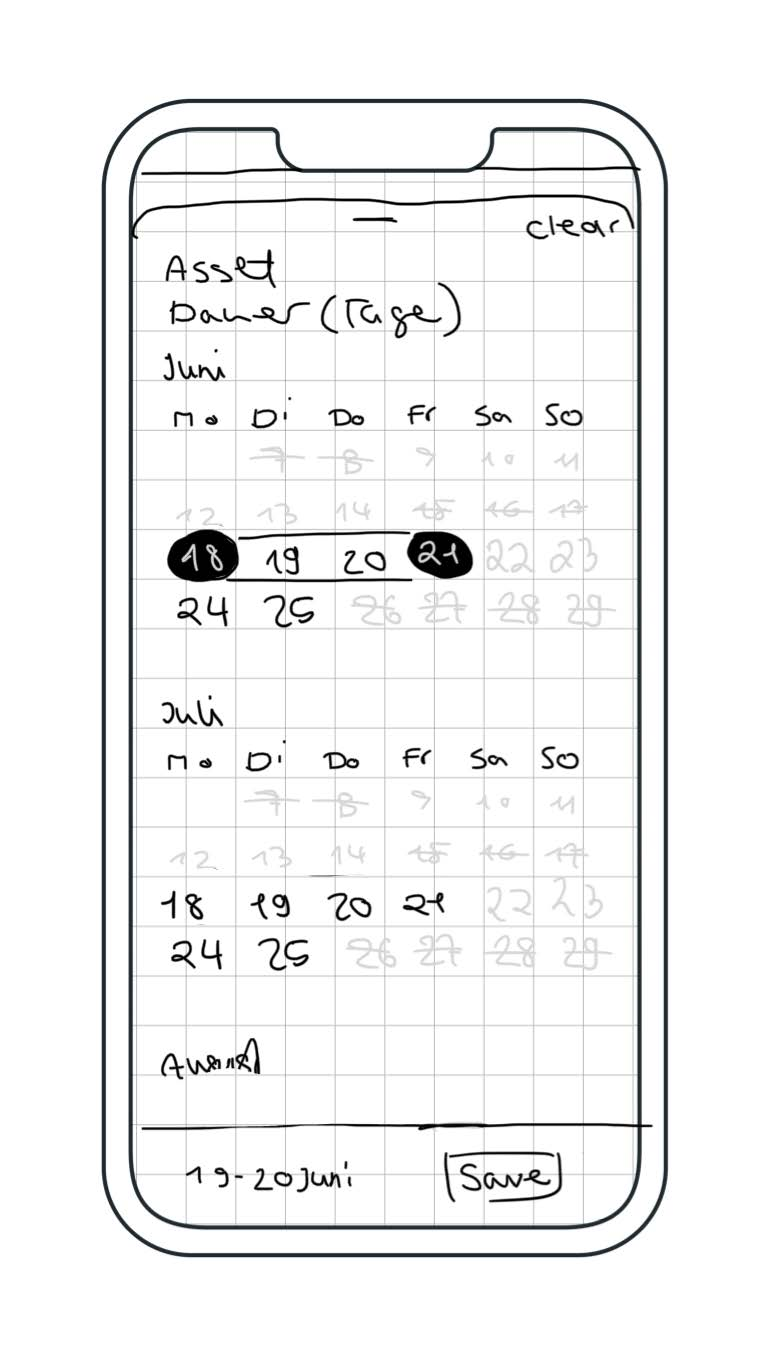
\includegraphics[scale=0.35]{Bilder/Mockups/Kalender.jpg}\hspace{2em}
    \caption{Skizzen der Kalenderkomponente in der mobilen Ansicht}
    \label{fig:kalender}
\end{figure}
\begin{figure}[h]
    \centering
    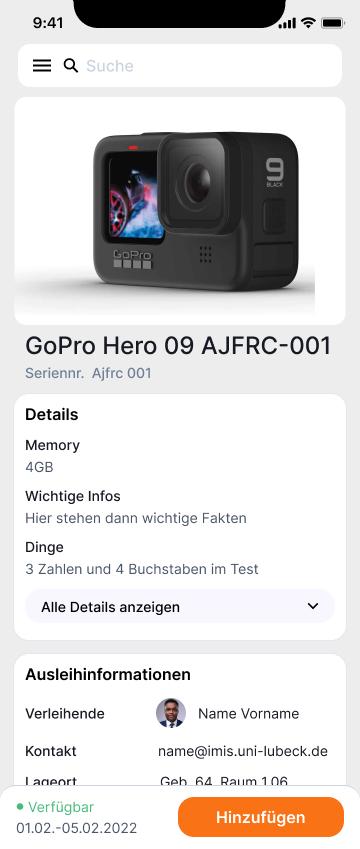
\includegraphics[scale=0.3]{Bilder/Prototyp/Neu/Datailansicht-1.png}\hspace{2em}
    \includegraphics[scale=0.3]{Bilder/Prototyp/Reservierung abschließen 3.png}
    \caption{Reservierung und Check-out in der mobilen Ansicht}
    \label{fig:p3}
\end{figure}